RelaySpec reuses a pretrained speculative drafter when its target is fine-tuned or replaced by a different model. We train linear maps that transform the new target's hidden states into inputs the existing drafter can use, while keeping the target and the original drafter weights frozen. The drafter uses these mapped features to propose tokens, and the new target verifies them. This lets us adapt the drafter to a changed target without retraining its prediction network. Our main implementation and experiments use DFlash~\citep{chen2026dflash}, so we describe its architecture and training procedures first, then apply the same construction to EAGLE-3.

\subsection{Adapting the drafter's inputs}
\label{sec:method-inputs}
We retain the drafter's $K$ target-layer inputs and place one map before each original fusion block~\citep{chen2026dflash}. DFlash uses $K=5$. Map $W_i$ connects the new target's selected feature stream $i$ to the corresponding original drafter input. The same map is applied at every token position. At position $t$, let $h_{i,t}\in\mathbb R^{d_t}$ be the new target's feature from selected layer $i$. A bias-free map $W_i\in\mathbb R^{d_r\times d_t}$ converts it to the width $d_r$ expected by the drafter. The frozen fusion block $F_i\in\mathbb R^{d_d\times d_r}$ projects it to the draft width $d_d$. The $K$ streams give the context
\begin{equation}
 \widehat c_t=N\!\left(\sum_{i=1}^{K}F_i W_i h_{i,t}\right),
 \label{eq:mapped-context}
\end{equation}
where $N$ is the original RMSNorm~\citep{zhang2019rmsnorm}. Only $W_1,\ldots,W_K$ are trained. The target, fusion projection, normalization, and draft transformer remain frozen. We also retain and freeze the original drafter's token embeddings and vocabulary output head.

After training, we multiply each learned matrix $W_i$ by its corresponding fusion block $F_i$ and join the $K$ products into one matrix:
\begin{equation}
 G=[F_1W_1\;\cdots\;F_KW_K]\in\mathbb R^{d_d\times Kd_t},
 \qquad \widehat c_t=N(G[h_{1,t};\ldots;h_{K,t}]).
 \label{eq:folded-fusion}
\end{equation}
The bracketed features are stacked into one vector. Block multiplication gives $G[h_{1,t};\ldots;h_{K,t}]=\sum_i F_iW_ih_{i,t}$, so one multiplication by $G$ replaces the separate map and fusion operations in exact arithmetic. The original normalization remains afterward. Figure~\ref{fig:relayspec-overview} shows both computations. We keep the maps linear because a linear map both changes the feature width and folds into the fusion projection. In our benchmarks a nonlinear alternative with more parameters does not improve on it, as Section~\ref{sec:ablation-capacity} reports.

\begin{figure}[!hb]
    \centering
    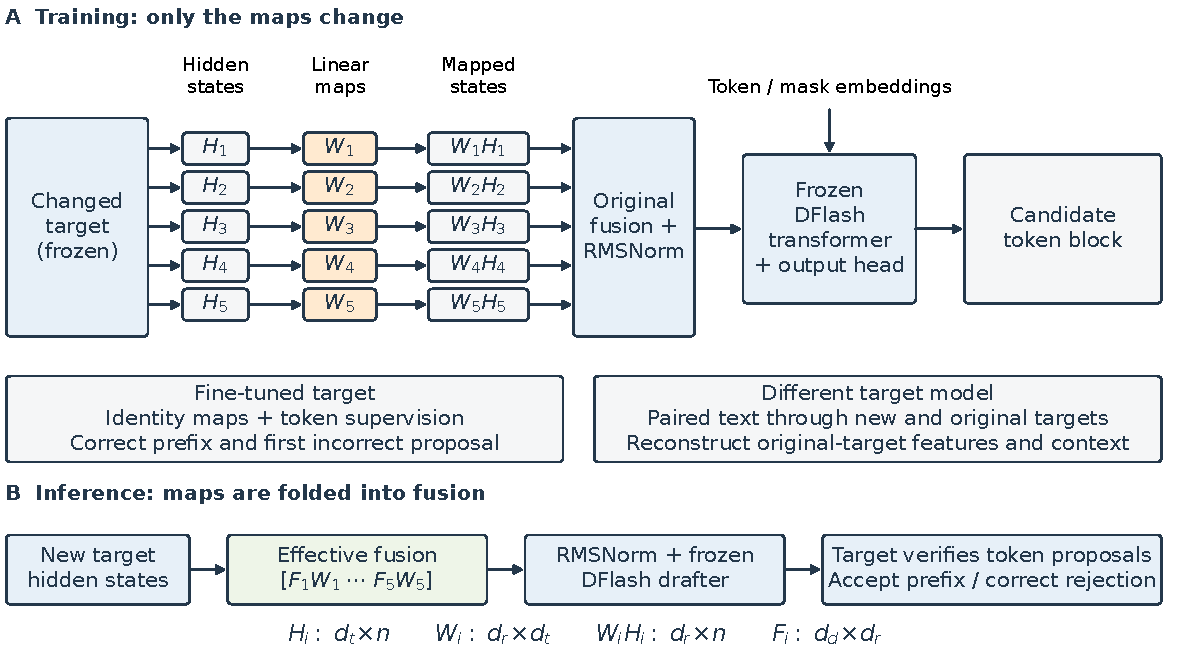
\includegraphics[width=\linewidth]{figures/relayspec_overview.pdf}
    \caption{RelaySpec training and inference. Orange maps are trainable and blue components are frozen. Each $H_i\in\mathbb R^{d_t\times n}$ holds $n$ context positions. For Qwen3-8B with the Qwen3-4B drafter, $d_t=4096$ and $d_r=d_d=2560$: maps are $2560\times4096$ and the combined projection is $2560\times20480$.}
    \label{fig:relayspec-overview}
\end{figure}


\subsection{Training for a LoRA-adapted target}
\label{sec:method-auf}
\textbf{Initialization.} When LoRA fine-tuning~\citep{hu2022lora} changes the target, its feature dimensions remain the same. We therefore initialize each map to the identity, $W_i=I$, so inserting the maps does not disrupt the existing drafter's behavior with the adapted target. At initialization, $F_iW_ih_{i,t}=F_ih_{i,t}$ for every input, so the maps leave the original computation unchanged. This preserves the starting behavior with the active LoRA target, not the behavior of the target before fine-tuning. Training then learns changes $\Delta_i=W_i-I$ that help the frozen drafter predict the adapted target's tokens.

\textbf{Training data.} We generate responses with the adapted target and save their tokens and hidden states. At sampled response positions, the drafter receives one known token followed by 15 masked positions to predict. Together they form a block of 16 tokens, matching the pretrained Qwen DFlash configuration~\citep{chen2026dflash}. We retain this block structure to adapt the existing drafter without changing its prediction procedure. Each block can use target features only from before its starting position. Following DFlash, attention connects positions within a block but not separate blocks~\citep{chen2026dflash}.

\textbf{Objective.} Because verification stops at the first rejected proposal, we supervise the correct prefix and the first incorrect prediction, excluding later positions. This is the accept-until-fail (AUF) objective~\citep{yang2026specauf}. For block $b$ and proposal position $j$, let $q_{bj}$ be the predicted token distribution, $y_{bj}$ the saved target token, and $m_{bj}$ a mask that excludes padding and non-response positions. We compute
\begin{equation}
 \begin{gathered}
 u_{bj}=\mathbf 1\!\left[\arg\max_v q_{bj}(v)=y_{bj}\ \text{or}\ m_{bj}=0\right],
 \qquad s_{bj}=\operatorname{stopgrad}\bigl({\textstyle\prod_{k<j}u_{bk}}\bigr),\\
 \mathcal L_{\mathrm{AUF}}
 =-\frac{\sum_{b,j}m_{bj}s_{bj}\log q_{bj}(y_{bj})}
 {\sum_{b,j}m_{bj}s_{bj}}.
 \end{gathered}
 \label{eq:auf-method}
\end{equation}
The product includes only earlier predictions, so the first failure still receives supervision. We recompute this mask from current predictions and hold it fixed during differentiation. Gradients pass through the frozen drafter to update the maps. We normalize the loss within each microbatch before averaging across accumulation steps and workers.

\subsection{Training for transfer across models}
\label{sec:method-mse}
\textbf{Initialization.} A drafter trained with one target expects that target's hidden states. Replacing the target can change both their dimensions and meaning. We therefore train the maps to reconstruct features from the original target, the model used to train the drafter. For this setting, we initialize the maps with independent Xavier-uniform values~\citep{glorot2010initialization}.

\textbf{Training data.} We generate responses with the new target, then run both targets causally on the same saved prompt and response to collect paired hidden states. The original target does not generate a separate response. With a shared tokenizer, both receive identical token IDs. When tokenizers differ, we pair only positions corresponding to the same text prefix. The original target is needed to prepare these training features, but is not used during adapted inference.

\textbf{Objective.} For example $b$ and position $t$, let $h_{bti}$ and $h^{(o)}_{bti}$ denote the paired new- and original-target features in stream $i$. The original features supply the context we aim to reconstruct:
\begin{equation}
 c^{(o)}_{bt}=N\!\left(\sum_{i=1}^{K}F_i h^{(o)}_{bti}\right).
 \label{eq:original-context}
\end{equation}
For $B$ examples, let $S_b$ contain the selected valid prompt and response positions in example $b$. Using relative squared error, we minimize
\begin{gather}
 D(u,v)=\frac{\lVert u-v\rVert_2^2}{\lVert v\rVert_2^2+\varepsilon},
 \qquad \varepsilon=10^{-6},
 \label{eq:relative-error}\\
 \mathcal L_{\mathrm{MSE}}
 =\frac1B\sum_{b=1}^{B}\frac1{|S_b|}\sum_{t\in S_b}
 \left[\frac1K\sum_{i=1}^{K}D(W_i h_{bti},h^{(o)}_{bti})
 +D(\widehat c_{bt},c^{(o)}_{bt})\right].
 \label{eq:mse-method}
\end{gather}
The first term averages reconstruction errors across the $K$ feature streams. The second reconstructs the combined context received by the draft layers. These two terms have equal weight. We exclude padding and average positions within each example before averaging examples. Unlike AUF, this objective trains the maps without passing gradients through the draft transformer. Dividing by each original vector's squared norm makes the error relative to its magnitude. The context term complements the layer terms because errors in different streams can interact when the fusion projection combines them. Reconstruction is a training objective, not a guarantee of accepted tokens, so we evaluate live decoding separately.

\subsection{Extension to EAGLE-3}
\label{sec:method-eagle}
The construction is not specific to DFlash. EAGLE-3 combines features from three target layers before autoregressive drafting~\citep{li2025eagle3}, so $K=3$. We place one map before each of those inputs and leave the original feature projection, prediction network, and autoregressive drafting procedure unchanged. The maps fold into that projection exactly as in Equation~\ref{eq:folded-fusion}, so inference again runs the original architecture with one updated projection.

We pair each setting with the same objective we use for DFlash. For a LoRA-adapted target the feature widths match, so the maps start at the identity and receive token supervision. Because EAGLE-3 drafts one token at a time instead of filling a masked block, we apply the accept-until-fail rule along its own recurrent path. At each sampled anchor the drafter predicts up to eight successive tokens, a position is supervised only when every earlier prediction was correct, and the first incorrect prediction is still supervised. A saved token continues a path only where it matches the greedy prediction. The frozen drafter carries a reduced vocabulary head, so a target token outside that head ends a path without contributing a loss term, and we normalize each example by its own count of supervised positions. For a replaced target the widths can differ, so the maps start at Xavier-uniform values and train by reconstruction using Equation~\ref{eq:mse-method}.

\subsection{Generation and verification}
\label{sec:method-generation}
The new target computes hidden states during prompt processing and proposal verification. We retain states from the committed prefix and map them into context for subsequent drafting. The frozen drafter proposes tokens, and the target verifies them using its existing decoding procedure. After verification, the decoder removes rejected speculative positions from the caches before the next drafting step. The original target is no longer needed to supply features during generation. Cross-tokenizer transfer additionally requires a proposal-conversion procedure, which the hidden-state maps do not provide.

\textbf{Greedy verification.} For greedy decoding, changing the drafter does not change the target's output if block verification makes the same choices as sequential target evaluation on identical prefixes. To see this, assume that the committed prefix matches autoregressive decoding. Each accepted proposal equals the target's next choice, and the first rejected proposal is replaced by that choice. If all proposals are accepted, the target supplies the next token. The extended prefix therefore still matches, and induction establishes the result for the complete sequence~\citep{leviathan2023speculative,chen2023sampling}. This argument assumes consistent token handling, stopping rules, and target evaluation.
